\documentclass[draft]{agujournal2019}
\usepackage{url} %this package should fix any errors with URLs in refs.
\usepackage{lineno}
\usepackage[inline]{trackchanges} %for better track changes. finalnew option will compile document with changes incorporated.
\usepackage{soul}
\linenumbers

\draftfalse

%% Enter journal name below.
%% Choose from this list of Journals:
%
% JGR: Atmospheres
% JGR: Biogeosciences
% JGR: Earth Surface
% JGR: Oceans
% JGR: Planets
% JGR: Solid Earth
% JGR: Space Physics
% Global Biogeochemical Cycles
% Geophysical Research Letters
% Paleoceanography and Paleoclimatology
% Radio Science
% Reviews of Geophysics
% Tectonics
% Space Weather
% Water Resources Research
% Geochemistry, Geophysics, Geosystems
% Journal of Advances in Modeling Earth Systems (JAMES)
% Earth's Future
% Earth and Space Science
% Geohealth
%

\journalname{Geochemistry, Geophysics, Geosystems}


\begin{document}


\title{Laurentia's continued motion into the Neoproterozoic: new paleomagnetic pole from the Jacobsville sandstone}


\authors{Yiming Zhang\textsuperscript{1}, Nicholas Swanson-Hysell\textsuperscript{1}, Blake Hodgin\textsuperscript{1}, James Pierce\textsuperscript{1}, Anthony Fuentes\textsuperscript{1}}


\affiliation{1}{Department of Earth and Planetary Science, University of California, Berkeley, CA, USA}
% \affiliation{2}{Second Affiliation}
% \affiliation{3}{Third Affiliation}
% \affiliation{4}{Fourth Affiliation}


\correspondingauthor{Yiming Zhang}{yimingzhang@berkeley.edu}


\begin{keypoints}
\item A new paleomagnetic pole has been developed from the ca.990 Ma Jacobsville Formation 
\item Laurentia plate continued to move after 
\item The new pole from the Jacobsville Formation indicates the Grenville Loop could be younger than thought
\end{keypoints}


\begin{abstract}
[ enter your Abstract here ]
\end{abstract}

\section*{Plain Language Summary}
[ enter your Plain Language Summary here or delete this section]


\section*{ABSTRACT}

The ca. 1.1 Ga North American Midcontinent Rift resulted in protracted magmatism and the associated deposition of sediments in the interior of Laurentia while the continent traveled rapidly from high to low latitudes. Coeval with the cessation of rifting and decreasing in the speed of plate motion is the ca. 1090-980 Ma Grenvillian Orogeny whose far-field stress is interpreted to have propagated into the interior of Laurentia and inverted the Midcontinent Rift, deforming the post-rift Jacobsville Formation. A lack of paleomagnetic record from the interior of Laurentia between the end of the Midcontinent Rift and the cooling of rocks associated with the Grenvillian Orogeny resulted in poorly constrained position and orientation of Laurentia for nearly 100 Myr. To fill this gap, we develop a new paleomagnetic pole from red beds of the Jacobsville Formation along 5 stratigraphic sections in Northern Michigan, US. Our high-resolution thermal demagnetization experiments successfully resolve primary magnetic remanence that pass a fold test and a conglomerate test. Our results agree with previous chemical demagnetization data but provide additional constraints on the shallowing of the inclinations and on the age of the pole once paired with max deposition ages developed from high-precision detrital zircon dating. Inclination shallowing corrected paleomagnetic pole position places Laurentia at low latitudes south of the Keweenawan Track ca. 990 Ma, confirming continued plate motion of Laurentia across the equator in the Late Mesoproterozoic to early Neoproterozoic. The new pole from the interior of Laurentia indicates the Grenville Loop poles are younger than previously thought.

\begin{keypoints}
\item Laurentia  
\item Inclination shallowing  
\item Paleogeography  
\item Grenville  
\item Keweenawan Superchron  
\item Red Bed 
\end{keypoints}

\begin{figure}
\noindent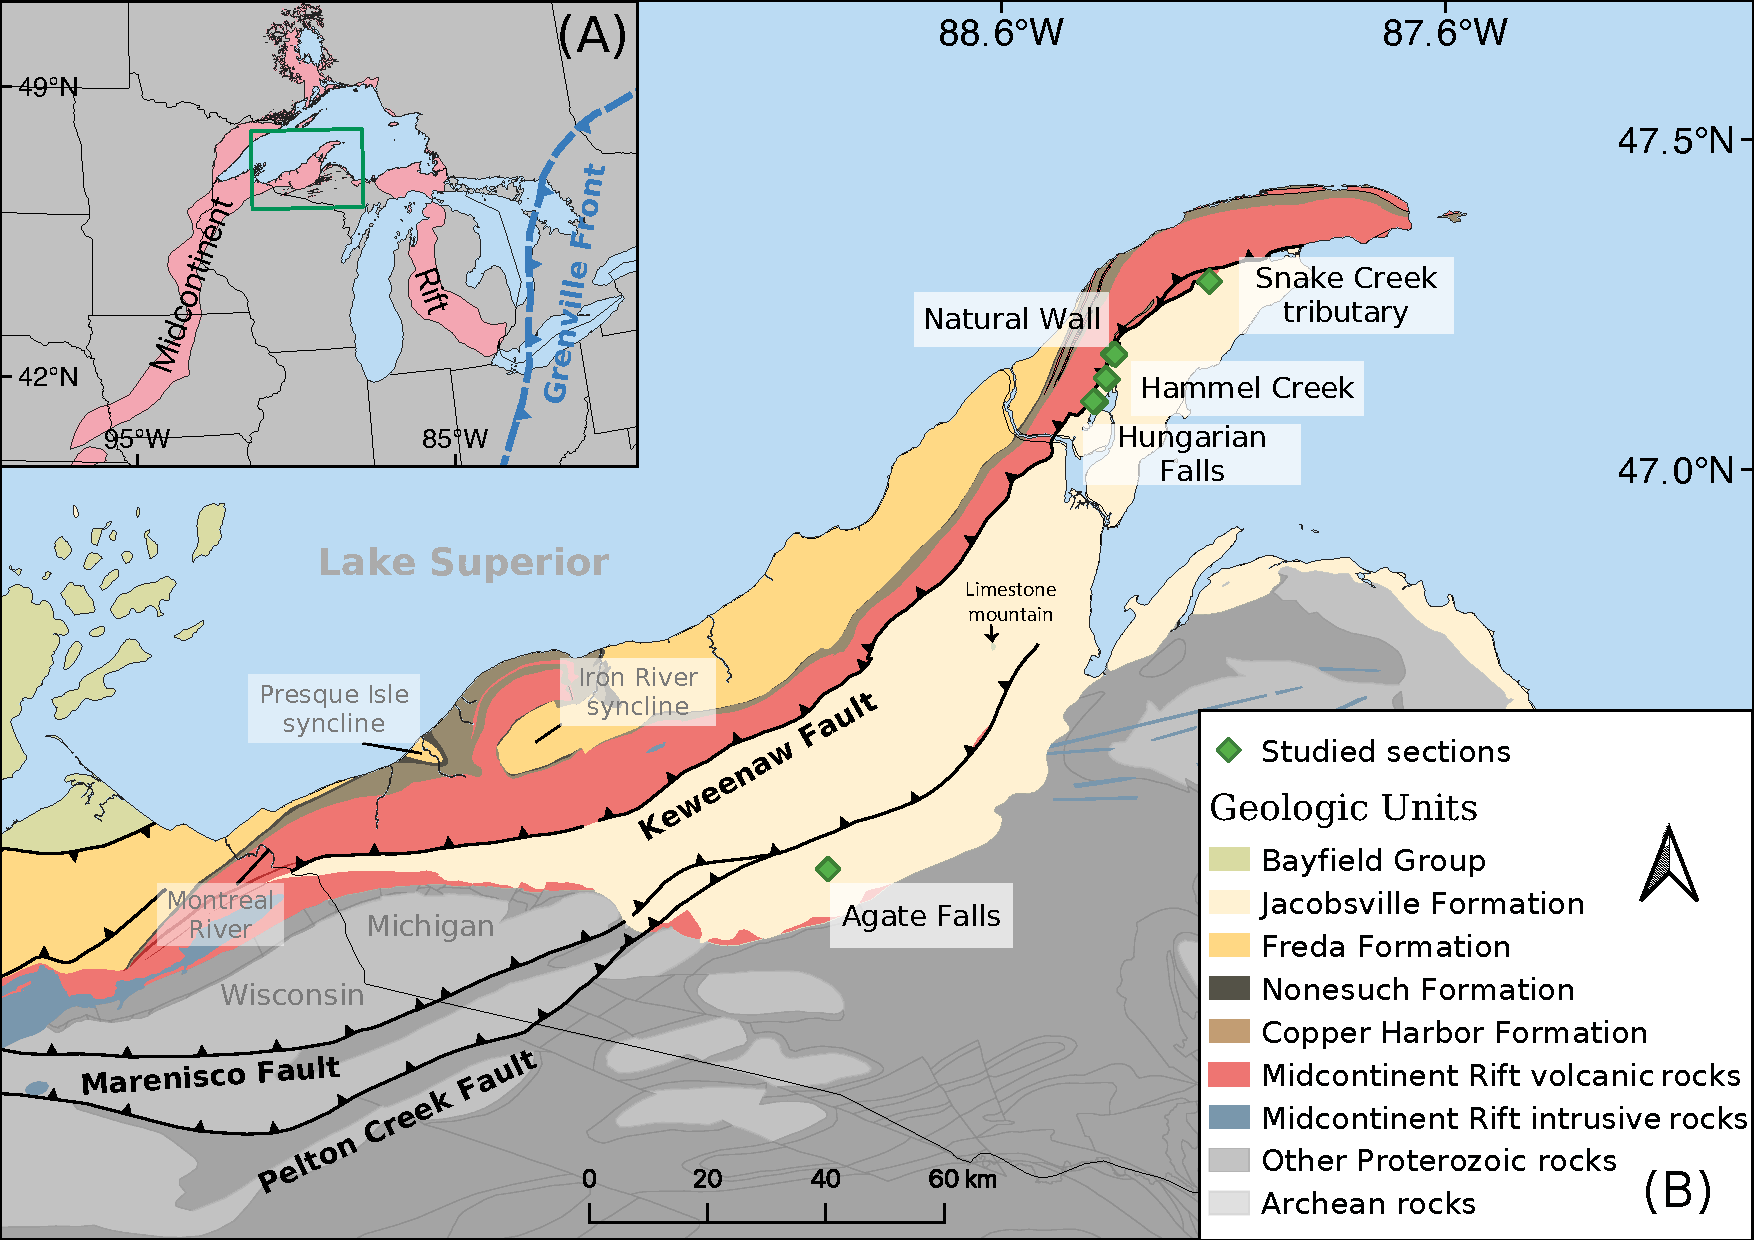
\includegraphics[width=\textwidth]{../Figures/Geologic_map.pdf}
\caption{caption}
\label{pngfiguresample}
\end{figure}

\section*{INTRODUCTION}

Paleomagnetic data for the Jacobsville Formation have led to a paleomagnetic pole position that appears to be a continuation of the Keweenawan Track from the Oronto Group poles (Roy and Robertson, 1978; Fig. 7; Table 4). As a result, its age has been interpolated to be latest Mesoproterozoic (e.g., 1020 Ma in Li et al., 2008) such that it was deposited prior to the ca. 1000 Ma Grenville loop poles. However, this age assignment has recently been questioned on the basis of laser-ablation–inductively cou- pled plasma–mass spectrometry (LA-ICP-MS) U-Pb detrital zircon dates from Jacobsville Sandstone samples. Malone et al. (2016) interpreted a maximum depositional age of 959 ± 19 Ma based on the weighted mean of the four youngest grains from 2050 LA-ICP-MS zircon dates. A similar age was proposed on the basis of the youngest LA-ICP-MS U-Pb dates in the study of Craddock et al. (2013). This young maximum interpreted age is intriguing because it suggests the unconformity above the Freda Sandstone spans at least 100 m.y. and was followed by continued sedimentation in the region long after rift activity. Nevertheless, the paleo- magnetic pole of the Jacobsville Sandstone (Roy and Robertson, 1978) appears to extend the Keweenawan Track from the Oronto Group poles in a manner that may be more consistent with deposition of the Jacobsville Formation in the late Mesoproterozoic. Given the conflict with this inferred age, the large uncertainty of individual LA-ICP-MS dates, and the pos- sibility of outlier dates in such a large data set, it is beneficial to interpret the age of the youngest Jacobsville zircons dated CA-ID-TIMS to obtain more precise constraints. Using CA-ID-TIMS, a recent study by Hodgin et al (2022) redefines the maximum deposition age of the Jacobsville Formation as ca. 993 Ma.


The extensive paleomagnetic studies of the well-preserved late Mesoproterozoic to Neoproterozoic rocks of North America have provided the central record for global paleogeography reconstruction during the assembly and rearrangement of the postulated supercontinent Rodinia. Paleomagnetic studies of rocks from Laurentia have led to a series of paleomagnetic poles that form an apparent polar wander path (APWP) known as the "Logan Loop" for the older high latitude poles at its apex that continues into the ``Keweenawan Track" of younger lower latitude poles that form a progression as the APWP heads toward the ``Grenville Loop" \citep{Swanson-Hysell2019a}. In particular, recent advances in pairing high-precision zircon U-Pb geochronology with high-quality paleomagnetic poles significantly improved the resolution of the Keweenawan Track and revealed Laurentia's rapid motion ($>$20 cm/yr) during the Midcontinent Rift magmatic activity from ca. 1110 Ma to ca. 1085 Ma \citep{Swanson-Hysell2019a}. 

As the Midcontinent Rift magmatic activity wanes its strength and evolved into a failed intracontinental rift, Laurentia experienced a long period of magmatic quiescence in its interior, where basin subsidence dominated the rift basin. This was followed by the Grenville Orogeny, causing the the inversion of the rift along thrust belts such as the Keweenaw Fault (Fig. xxx). The lack of extensive magmatism from ca.1080 Ma to ca. 980 Ma in the Laurentia interior resulted in a significant gap (for at least 50 myr) of paleomagnetic poles between the Keweenawan Track (developed from interior Laurentia igneous and sedimentary rocks) and the Grenville Loop (poles developed from the Grenville Province rocks) (Fig. xxx; \cite{Swanson-Hysell2019a}).  

Due to the lack of pmag records from the interior Laurentia, various hypotheses for the spatial relationship between the end of the Keweenawan Track and the Grenville Loop have been debated. One model argues for that the difference in pole locations indicates that the Grenville Province was once thousands of kilometers away from Interior Laurentia and was progressively approaching the southern margin of Laurentia in the late Mesoproterozoic \citep{Halls2015}. A corollary of this hypothesis is that there had to be a 4000 km shortening during the Grenville orogeny - colliding Amazonia-Laurentia. The other model favors that the Grenville Loop is a continuation of the Keweenawan Track - that the southerly continental drift of Laurentia continued across the equator onto the southern hemisphere from ca. 1070 Ma to ca.1000 Ma. and  approached this problem by developing data from metamorphosed dike and anorthosite and argued for Grenville  

Paleomagnetic poles from the interior of Laurentia during the quiescence magmatism period is thus crucial for reconcile the discordant paleomagnetic poles of the Keweenawan Track and the Grenville Loop. The
%Q: what are you using the poles from rocks that we know are from the Laurentia interior? (outside of the Grenville package?)

This new age constraint on the Jacobsville provides crucial insight into the tectonic evolution of the Midcontinent Rift and the inversion of the extensional region into a compressional region due to the Grenville orogen. It also makes the Jacobsville sandstone a unique opportunity to investigate Laurentia's paleogeographical position at ca. 1 Ga as a long period of magmatic quiescence for $\sim$50 myr precedes Jacobsville deposition left a gap in Laurentia apparent polar wander path between the Keweenawan Track and the Grenville Loop (Fig. xxx). 

Jacobsville sedimentation was preceded by a long period of volcanic and tectonic quiescence and cratonic stability so that bedrock surfaces became blanketed by paleosol and a surface of chemically resistant debris was dominated by quartz and iron-formation. 

Previous paleomagnetic study on the red beds within the Jacobsville by \cite{Roy1978a} observed different components using AF, thermal, and chemical demagnetizations. Recognized dual polarities and recognized the complex remanence acquisition of red beds which lead to three isolated remanence components from the Jacobsville. However, that study did not recognize the problem of inclination shallowing and did not apply correction factor on the results. Moreover, the course demagnetization steps during thermal demagnetization would have had limited resolution for distinguishing the depositional remanent magnetization (DRM) and secondary chemical remanent magnetization (CRM) which have recently been shown to unblock over a narrow temperature window \cite{Swanson-Hysell2019b}. 

In this study, we use fine-grained to silt-sized, hematite rich red beds from xxx sections along the Keweenaw Peninsula, Michigan with the goal of obtaining high-quality paleomagnetic pole from the jacobsville formation that is corrected for inclination shallowing problem and to investigate the connection between the Keweenawan Track and the Grenville Loop of the Laurentia APWP during the late Mesoproterozoic to the Neoproterozoic. 

\section*{GEOLOGIC SETTINGS}


The Jacobsville sandstone is 
\cite{Kalliokoski1982a} In the Lake Superior syncline the Jacobsville Sandstone is a thick (+900m) fluvial sequence of feldspathic and quartzose sandstones, conglomerates, siltstones, and shales, completely devoid of lava flows or cross-cutting dikes. On the north and south sides of Lake Superior, most of the sandstone occurs as inward-dipping, fault-bounded wedges, separated by regional faults from the Oronto and Bayfield Groups of similar red sandstones, situated on the inner side of the syncline. 

With its age being long debated through the past decades, recently detrital zircon work by \cite{Malone2016a} and \Hodgin{2021a} settled that the maximum deposition age of the Jacobsville sandstone  is 980 Ma, indicating the deposition of the Jacobsville predate or the upper Jacobsville overlaps with the Rigolet phase of the Grenville orogeny. The upper age of the Jacobsville is xxx Ma.


Keweenaw Fault motion post dating Jacobsville in the footwall
Youngest DZ from jacobsvill eis about 993 Ma (sandstone creek, about a few hundred meters from the fault). 
directly above pmag sampling at Agate falls grain B geochron date is (z2, s226, about 1000 Ma grain)

jacobsville (985.5 from calcite in the fault and <993 from zircons) 

Blake's current tectonic model: after MCR volcanics ca. 1084 Ma emplacement follows the deposition of the sediments (Oronto Group) copper harbor conglomerate, Nonesuch formation and the Freda formation. Then the Grenville orogenesis took off with the Ottawan phase from 1020 Ma - 10?? Ma and the Rigolet phase from 995-980 Ma. Paleosol development and the unconformity between the Jacobsville and the volcanics indicate a prolonged period of gap during which the Oronto Group in the backbulge basin where they were deposited were lost, resulting in younger Jacobsville deposition directly on top of the volcanics. The fact that in the Jacobsville has conglomerate and sandstone and siltstone facies in them supports sediment input from the eroded Oronto Group. This indicate the older boundary of the Jacobsville deposition might be closer to the Rigolet Phase than the Ottawan phase. The younger age boundary of the Jacobsville is well defined - given that the maximum deposition age from the zircons of the Jacobsville is 993 Ma and the calcite on the Keweenaw Fault is 985.5 Ma, the deposition of at least the upper portion of the Jacobsville is well constrained to be between 993 and 985 Ma. The deposition of Jacobsville in the back bulge in Laurentia interior is related to the far-field compression caused by the Grenville Orogeny. 

This makes the Jacobsville sandstone one unique opportunity to acquire a paleomagnetic pole position within the gap between the 

\subsection{Jacobsville stratigraphy}

Along the south shore of Lake Superior, the Keweenawan Supergroup overlies Paleoproterozoic basement and consists of ~5 km of rift-related volcanic rocks that are conformably overlain by ~4 km of conglomerate, siltstone, and sandstone of the Oronto Group (Cannon et al., 1996). The uppermost unit of the Keweenawan Supergroup is the Jacobsville Sandstone, which consists of up to ~1 km of fluvial deposits that are more quartz-rich than the Oronto Group (Fig. 1; Kalliokoski, 1982). The Jacobsville Sandstone unconformably overlies Archean and Paleoproterozoic basement as well as Midcontinent Rift volcanic and sedimentary rocks in northern Michigan (Fig. 1; Cannon et al., 1993; Ojakangas et al., 2001). The overall extent of the Jacobsville Sandstone has been mapped along the southern shore of Lake Superior, from west to east - the Keweenaw Peninsula of northern Michigan to Sault Ste Marie, Canada (Fig. \ref{}). The Jacobsville Sandstone is unconformably overlain by the Cambrian Munising Formation (Hamblin, 1958).

The Keweenaw Fault is a north to northwest-dipping thrust that extends ~250 km from the tip of the Keweenaw Peninsula in northern Michigan southeastward to a termination in northeastern Wisconsin (Fig. 1; Cannon et al., 1996; Cannon and Nicholson, 2001). Thrust faults parallel to the Keweenaw Fault include the northwest-dipping Marenisco and Pelton Creek faults (Fig. 1). Similarly-oriented thrusts continue southwestward through northern Wisconsin and eastern Minnesota (Ojakangas et al., 2001), and eastward below Lake Superior, where they are interpreted to join mapped thrust faults in southern Ontario (Fig. 1; Manson and Halls, 1994; Ojakangas et al., 2001). Rock units adjacent to these regional thrusts have been moderately to intensely folded. In northern Michigan, the typically shallowly-dipping Jacobsville Sandstone has sub-vertical to overturned beds in the immediate footwall of the Keweenaw Fault (Irving and Chamberlin, 1885; Cannon and Nicholson, 2001). Near the Keweenaw Fault, Jacobsville Sandstone consists of quartz-rich, cross-bedded, medium-grained sandstone, locally abundant clast-supported conglomerate, and minor interbeds of red micaceous siltstone. The conglomerate contains volcanic clasts likely derived from uplifted Midcontinent Rift volcanics (Irving and Chamberlin, 1885; Brojanigo, 1984). Clast provenance in Jacobsville conglomerates includes Paleoproterozoic lithologies, such as vein quartz and iron formation clasts, which are abundant in southern exposures (Hamblin, 1958; Kalliokoski, 1982). Occurrence of conglomerates in proximity to the Keweenaw, Marenisco, and Pelton Creek thrusts is interpreted to represent syn-depositional development of local relief (Kalliokoski, 1982; Hedgman, 1992). 

It has been interpreted that the Jacobsville Sandstone is equivalent to the Bayfield Group in northern Wisconsin, and the Fond Du Lac and Hinckley formations in Minnesota. Their shared lithofacies of basal conglomerate, cross-bedded fluvial fine to medium grained sandstone, and interbedded red micaceous siltstone could  support the interpretation that these sedimentary rocks formed during a common period of post-rift basin formation following rift-related magmatism of the MCR. 

Red beds, particular fine-grained siltstone beds have been shown to be good paleomagnetic recorders, preserving magnetic remanence for up to billions of years. Occurrence of red siltstone beds have been reported in the Jacobsville Sandstone, particularly in the upper sections near Keweenaw Fault (e.g. Hamblin1958a, Irving1885a). They typically in the field are brick-red to dark-red, find-grained arenite to arkosic sandstone and siltstone. Minor grey reduction spots can be found. rounded detrital mica grains up to 5mm? size can be found commonly within very fine, fissile siltstone and shaly strata. 


\subsubsection{Paleomagnetic sample sites}
Agate Falls
A MDA of --- Ma was obtained from this site by Hodgin2021a. 

Natural Wall
A MDA of --- Ma was obtained from this site by Hodgin2021a

Snake Creek
A MDA of --- Ma was obtained from this site by Hodgin2021a

JK creek
A MDA of --- Ma was obtained from this site by Hodgin2021a



\cite{Roy1978a} sampled 37 sites across a lateral distance of 


\section*{METHODS and RESULTS}



\section*{DISCUSSION}

paleomagnetic mean pole of the Jacobsville Sandstone and the age

inclination shallowing correction of the Jacobsville Sandstone

magnetic reversal during the Jacobsville and the Maya Superchron

Implication on the crustal shortening of the Rigolet phase of the Grenville Orogeny

Warnock on the age of magnetization on the Haliburton pole: based on the very coarse thermal demagnetization steps Warnock2000a assigned that all of the primary magnetite components unblocked above 550 \textdegree C, with an uncertainty of 555 \textdegree C $\pm$ 5\textdegree C. Using a thermal history model that combines U-Pb titanite ages, hornblende and biotite Ar/Ar ages and just by merely compare the thermal history model with the assigned narrow magnetite unblocking temperature range, the authors assigned the age of the magnetization to be 1015 $\pm$ 15 Ma. 

It is important to note that the result Ar ages of the hornblende and biotite are 983 $\pm$ 8 Ma, 996 $\pm$ 8 Ma, and 998 $\pm$ 8 for hornblende with unblocking temperature of 530 $\pm$ 40\textdegree C, consistent across metamorphic terranes (Bancroft). And the biotite Ar ages are 910 $\pm$ 7 Ma, 891 $\pm$ 7 Ma, corresponding to unblocking temperature of 280 $\pm$ 40\textdegree C. 

More, the thermal demagnetization plots shown in Warnock2000a suggest that the magnetite unblocking lower temperature boundary can be around 500\textdegree C, lower than 555 $\pm$ 5\textdegree C. In addition, given the case that the rocks underwent uniform rate of cooling due to post-formation uplifting, a slow cooling effect from 555\textdegree C to 300\textdegree C from 990 Ma to 900 Ma allows for a scenario where the magnetite remament magnetization that appear to have a 555\textdegree C unblocking temperature in lab was acquired through a period of --- myr cooling though 500\textdegree C during uplifting. In this case, the magnetite remanence acquisition can be interpreted to be closer to the biotite Ar age than previously thought. Therefore, the Haliburton intrusion pole could be interpreted to be a post Rigolet orogenic activity phase magnetization acquisition, and the apparent discrepancy between the Haliburton pole and the Jacobsville pole can be explained by Laurentia's whole plate motion after the Grenvillian orogeny from 990 Ma to 900 Ma. One corollary of such scenario is that Laurentia underwent plate motion at a rate of ---\textdegree/myr, which is similar to that of today's tectonic plate motion. 

Crucial link between the Keweenawan Track and the Grenville Loop



\acknowledgments
Enter acknowledgments, including your data availability statement, here.


\bibliography{YZ_ref}




\end{document}
